\chapter{Introduction}

\label{chapter:introduction}

This is the introductory chapter. I am going to tell you all the background and definitions you need to understand the material in Chapter~\ref{chapter:chapter2} and Chapter~\ref{chapter:chapter3}).


\section{First Background Section }



\subsection{Something About this}

%Here is some text. And it describes some evidence that is found in
%Figure~\ref{elephantfig}.
%
%
%\begin{figure}[htb!]
%\begin{center}
%  \fbox{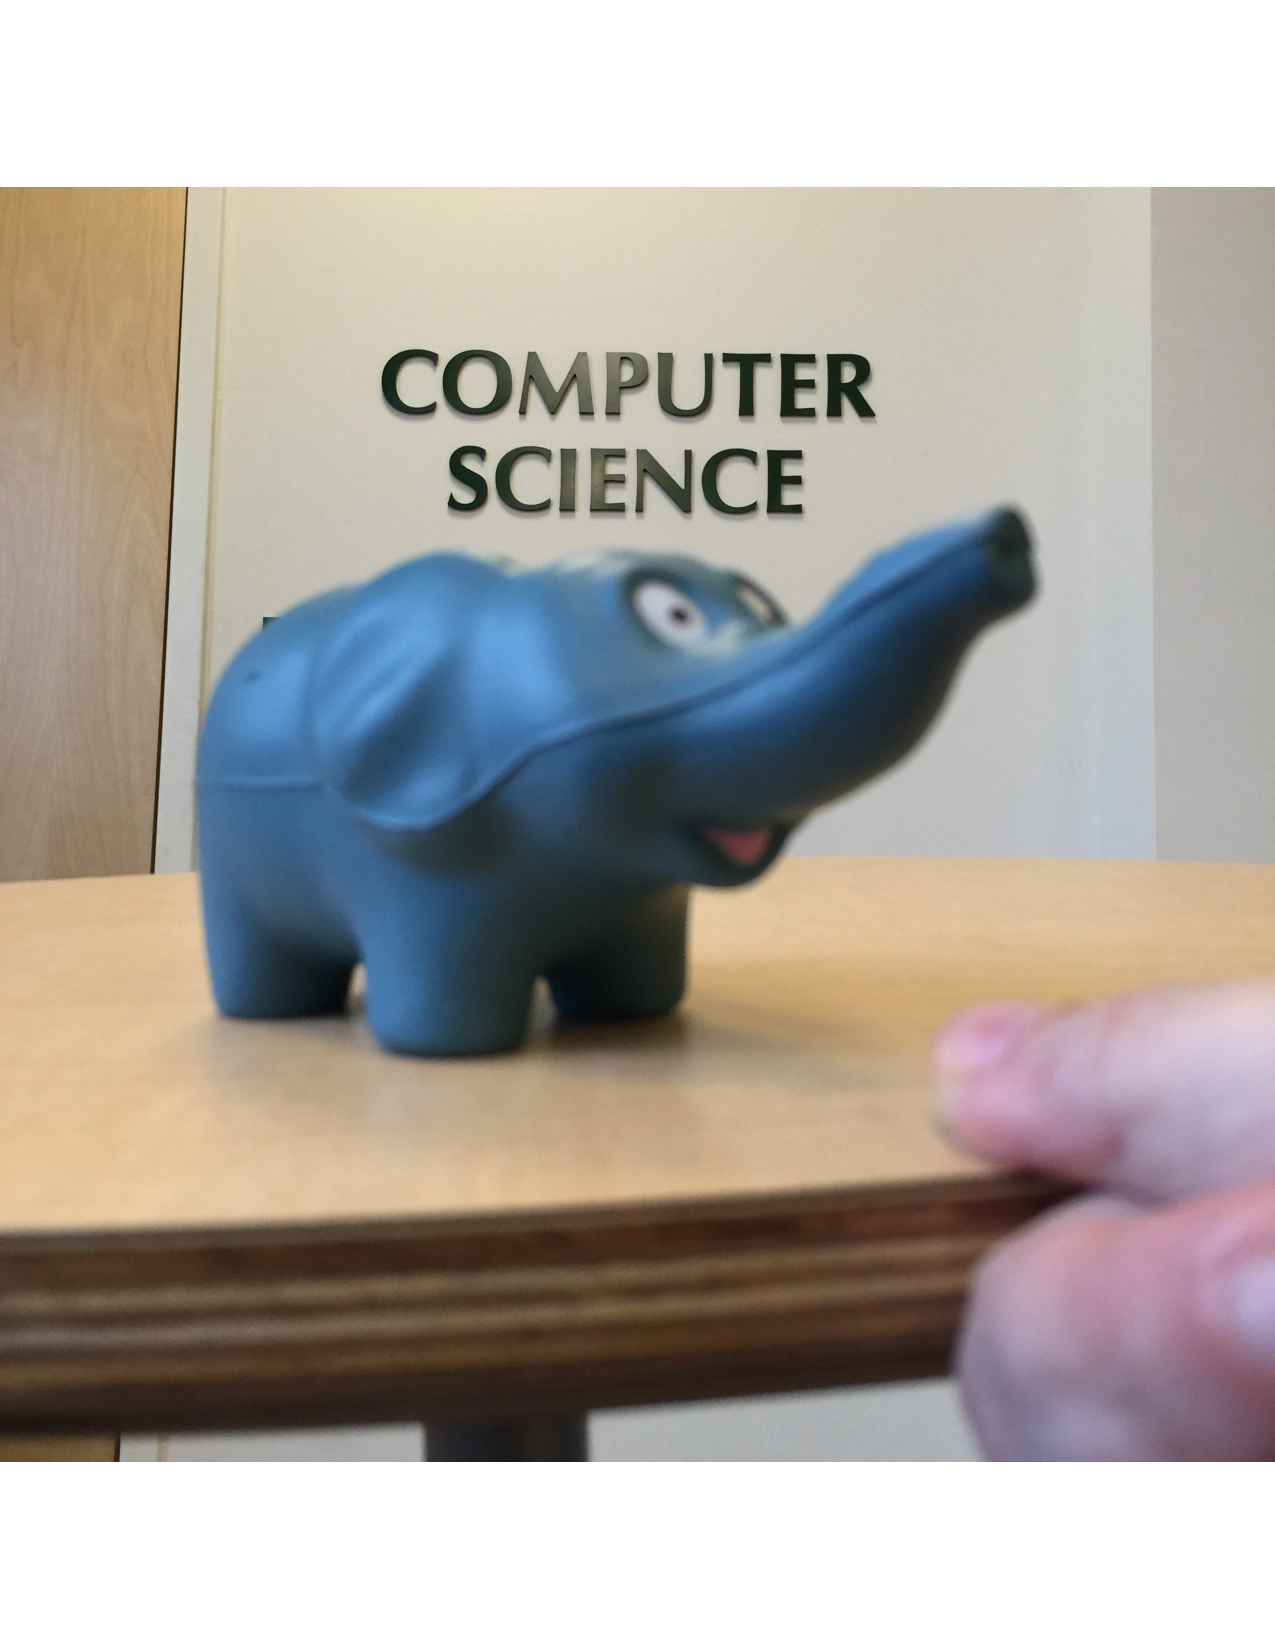
\includegraphics[height=4.5in]{cs-focus.pdf}}
%   \caption{The footprints in the margarine}
%   \label{elephantfig}
% \end{center}
%\end{figure}
%
%
%\section{Outline of This Work}
%
%Following is the  outline  of individual chapters in this thesis.
%
%In Chapter 2, we show the trunk.
%
%In Chapter 3, we discuss the search space. 
%
%Finally in Chapter 4, we discuss the results and summarize the key
%findings of this thesis followed by possible directions of future
%work.
